\documentclass{article}
\usepackage[utf8]{inputenc}
\usepackage{graphicx}
\usepackage[colorlinks=false,
            linkcolor=blue]{hyperref}
\usepackage{longtable}

\title{Recognizing Choice of Spelling with LLMs}
\author{David Meltzer}
%\date{Date of Document}

\begin{document}

\maketitle

\begin{abstract}
In this report we will investigate the ability of GPT-4 to learn a classification task from in-context examples.
Specifically, we will teach GPT-4 to classify sentences as either using American English or British English spelling.
We use ChatGPT and Claude to generate our dataset of examples.
We test to what extent GPT-4 is able to both identify the classification rule and to actually perform the classification in practice.
In particular, we will measure how GPT-4's performance changes as a function of the number of in-context examples provided to the model. 
We see that model performance generally improves as we increase the number of examples, if we also ask the model to provide its reasoning.

\end{abstract}

\section{Introduction}
Can we use in-context learning to teach an LLM a new task?
In this report we investigate this problem in the context of teaching an LLM to distinguish between American English and British English spellings.
This can be a difficult task because the difference between the two spellings can be fairly small and correspond to just changing one letter.
Because the difference is small, we see that the model only learns the classification rule when it is provided with enough examples.
If the model is not provided with enough examples, it may be mislead by other differences between the sentences, for example whether the sentence is describing something positive or negative or if the sentence is describing something that has already occurred or is presently happening.

\section{Set-Up}
\label{sec:setup}
To generate our dataset we use two LLMs, ChatGPT-4 and Claude. 
We started by prompting ChatGPT-4 to generate a list of words whose spelling differs between American and British English.
Specifically, ChatGPT generated a list of tuples where the first element is the American English spelling and the second element is the British English spelling.
We sometimes found that ChatGPT generated words whose spelling appeared to be archaic and no longer in use, e.g. it generated the pair (``monolog", ``monologue").
While the ``log" ending is common in American English for other words, e.g. ``analog", the spelling ``monolog" does not appear to be in use anymore, so we removed this pair. 
Similarly, we also removed the pair (``jail", ``gaol"), since ``gaol" appears to be a dated spelling.
As a disclaimer though, there may be other archaic spellings in either American or British English which I missed.
The full list of words can be found in Table \ref{table:spelling_differences}.

To generate sentences, we then gave ChatGPT and Claude the following prompt:
\begin{center}
\begin{quote}
   ``\{\{\{List of tuples\}\}\}
\\[10pt]    
The first element of each tuple is the American spelling and the second element is the British spelling. For each tuple, and for each element of the tuple, can you form a sentence using either American or British spelling, depending on which word you chose. Do not use the same exact sentence for the American and British spelling of the word, try to be more creative and make them distinct.
\\[5pt]   
Format the final result as a list of tuples where the first element of the tuple is the sentence and the second element is True if you use American spelling and False if you use British spelling."
\end{quote}
\end{center}
Using this prompt, we created two datasets, one generated using ChatGPT-4 and the other generated using Claude. 
In practice, we did not use every sentence in the dataset. Instead we shuffled the dataset and chose the first 20 sentences to be our candidate in-context examples and we chose the next 50 sentences to be our evaluation set. The actual choice of sentences included in our prompt and evaluation sets can be found in Tables \ref{table:sentences1}-\ref{table:sentences4} for GPT-4 and Claude-generated examples. Given more time, it would be interesting to test the LLMs on larger datasets to get a better measure of their performance.

When asking the model to perform the classification, we considered two different system messages for GPT-4. In the first system message we asked the model to explain its reasoning explicitly:
\begin{center}
\begin{quote}
You have a series of input and output pairs. The input is a sentence and the output is either True or False.
Find a general rule to explain the pattern of input/output pairs. Explain your reasoning step by step.
The prediction for the last example should be the string `True' or `False' and nothing else.
Output the result in the following format:

REASONING: \{Put your reasoning here\} \textbackslash n
PREDICTION: \{prediction\}
\end{quote}
\end{center}
In the second prompt, we just ask the model to give a prediction and nothing more:
\begin{center}
\begin{quote}
You have a series of input and output pairs. The input is a sentence and the output is either True or False.
Find a general rule to explain the pattern of input/output pairs.
The prediction for the last example should be the string `True' or `False' and nothing else.
\end{quote}
\end{center}
For the most part, GPT-4 understands the instructions and follows the format prescribed. However, there were a few cases where the model outputs the prediction and then adds additional explanations later. For the moment, we mark any incorrectly formatted prediction as simply being incorrect, but in principle we should be more lenient and try to parse the output further.

\section{Analysis}
\begin{figure}
\centering
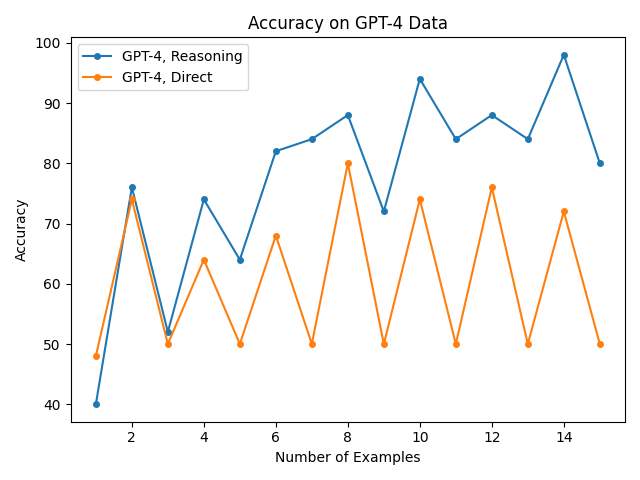
\includegraphics[scale=.6]{./figures/accuracy_GPT.png}
\caption{GPT-4's accuracy on the ChatGPT-generated dataset as a function of the number of in-context examples.}
\label{plot:accuracy_GPT}
\end{figure}

Now we can see how well GPT-4 learns our classification problem. In Figure \ref{plot:accuracy_GPT} we plot the accuracy of GPT-4 on the ChatGPT-4 generated dataset as a function of the number of in-context examples. 
In Figure \ref{plot:accuracy_claude} we make the same plot for the Claude generated dataset. In all cases, we take the first $k$ examples in the prompt dataset.

We can make a few observations. 
The first is that GPT-4 appears to be better at classifying sentences in the GPT-4 generated dataset than in the Claude-generated dataset.
In particular, for the GPT-4 generated dataset we get above 90\% accuracy with 10 in-context examples, while for the Claude-generated dataset we get around 70\% accuracy with 15 in-context examples.
However, it is possible we would get above $90\%$ accuracy on the Claude-generated dataset if we used even more in-context examples.

\begin{figure}
\centering
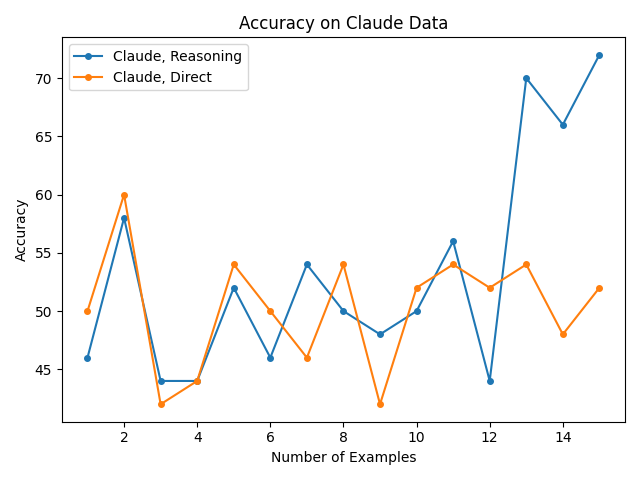
\includegraphics[scale=.6]{./figures/accuracy_claude.png}
\caption{GPT-4's accuracy on the ChatGPT-generated dataset as a function of the number of in-context examples.}
\label{plot:accuracy_claude}
\end{figure}

The reason GPT-4 is better able to classify the ChatGPT-4 generated dataset is likely due to a mistake in how we organized the data.
The prompt set for the ChatGPT generated dataset involves alternating pairs of True and False examples, where the first example in each pair uses the American spelling of a word and the next example uses the British spelling of the same word, see Table \ref{table:sentences1}.
Therefore, given these prompts, GPT-4 can quickly learn the classification criterion once it has seen a few complete pairs.

This also explains why the orange line in Figure \ref{plot:accuracy_GPT} (when we do not ask the model to reason) is oscillating. 
When we have an even number of examples, we always have pairs of sentences which share a common word that is spelled differently in American and British English.
Therefore, when we have an even number of examples, GPT-4 has a very clear signal about what the classification rule is. 
However, if we have an odd number of examples, we no longer have a perfect pairing between American and British spellings of the same word.
The fact that this odd sentence out is also the last one may also explain why the accuracy decreases significantly whenever we have an odd number of examples.
The decrease in performance is lessened when we also ask GPT-4 to explicitly reason about the input/output pairs (see the blue line in Figure \ref{plot:accuracy_GPT}), but we still notice dips when we have an odd number of examples.

For the Claude-generated dataset, the examples were shuffled and we do not have alternating pairs of True/False examples involving different spellings of the same word, see Table \ref{table:sentences3}.
In this case, the model needs to see more examples to determine the classification rule.
Although our original goal in generating the two datasets was to see if GPT-4 is better able to classify ChatGPT-4 generated data, as opposed to data generated via a different LLM, the two datasets instead let us see how the model's performance depends on the formatting and quality of the prompts.

\begin{figure}[ht]
\centering
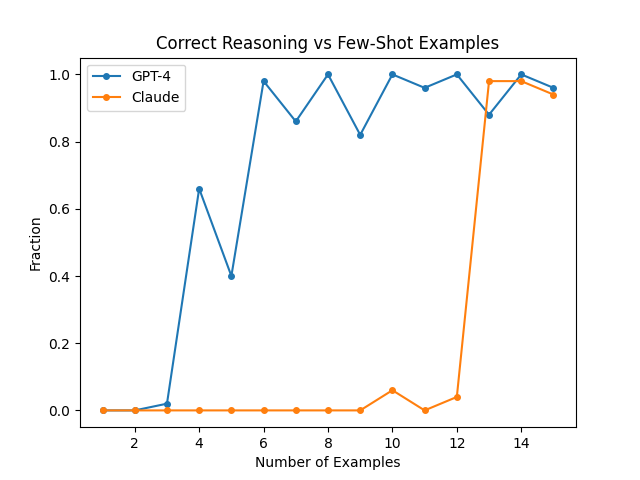
\includegraphics[scale=.6]{./figures/reasoning_plot.png}
\caption{Charting GPT-4's reasoning as a function of the number of in-context examples}
\label{plot:reasoning}
\end{figure}

We can also note that asking the model to reason about the problem generally improves its accuracy on both datasets. The improvement on the ChatGPT-generated dataset is noticeable when we have at least 4 in-context examples, while the improvement on the Claude-generated dataset is delayed and we see noticeable improvement when we have at least 13 in-context examples.

To understand the effect of reasoning on GPT-4's classification ability, we will study how often GPT-4's responses include the words ``American" and ``British".
In Figure \ref{plot:reasoning}, we plot the fraction of responses that include these words on the two evaluation datasets.
We see that as we increase the number of in-context examples, the model is better able to identify the classification rule.
In particular, on the ChatGPT generated dataset, GPT-4's response includes ``American" and ``British" in over half the responses once we have 4 in-context examples and these words appear in every response when we have 8, 10, 12, or 14 in-context examples.
On the Claude-generated dataset, GPT-4's response includes the strings ``American" and ``British" in almost every response once we have at least 13 examples. 
This is also the point where GPT-4's accuracy on the Claude generated dataset increases significantly, see Figure \ref{plot:accuracy_claude}.
%Of course, it would be interesting to study this pattern as we add more examples for both datasets.

Finally, we can study at what point the model learns the classification rule when it is given several in-context examples, without asking the model to perform any additional classification.
That is, we are seeing at what point GPT-4 can learn the classification rule, even if it cannot always apply it in practice. 
We prompt GPT-4 with the following system message:
\begin{center}
\begin{quote}
You have a series of input and output pairs. The input is a sentence and the output is either True or False.
Find a general rule to explain the pattern of input/output pairs.
Output the result in the following format:

REASONING: {Put your reasoning here}
\end{quote}
\end{center}

The results for the GPT-generated data are shown in Table \ref{tab:gpt_responses}.
We see that after just two examples, the model is able to correctly determine the classification criterion.
However, from our previous results, we know that GPT-4 only achieves an accuracy above \>90\% when we include at least 10 in-context examples.
Therefore, it appears that although the model can fairly quickly understand the classification problem, it struggles to consistently apply it to new sentences if we do not provide enough in-context examples.
We can likely improve GPT-4's performance on the GPT-generated data if we performed further prompt engineering.

The results for the Claude-generated data are shown in Table \ref{tab:claude_responses}.
Here the problem is significantly more difficult since, due to how we shuffled the data, we need at least 5 in-context examples before we see a single ``False" example. 
However, this cannot entirely explain the difference in GPT-4's performance on our two datasets.
For example, when we include 10 in-context examples from the Claude-dataset, GPT-4 is still not able to determine the correct classification criterion, even though we have 6 examples with American spelling and 4 examples with British spelling.
Instead, it is only once we include 13 in-context examples (8 American spellings, 5 British spellings) that GPT-4 is able to determine the pattern.
This again matches up with when GPT-4 is able to correctly classify examples in this dataset.

It would naturally be interesting to investigate this problem further and understand under what circumstances GPT-4 is able to consistently learn and apply a classification rule at the same time.
For example, is the fact that GPT-4 can learn the classification rule for the ChatGPT dataset, but not immediately apply it, because the prompts were organized in alternating pairs (which makes the problem simpler) or because applying a classification rule consistently requires that we have more in-context examples?
As mentioned earlier, it may also be interesting to explore how the source of the data, i.e. which LLM we choose to generate vs classify the data, affects our results.

%We can see a potentially interesting pattern. For the GPT-4 generated dataset, where the examples are not shuffled, GPT-4 can determine the classification problem with just two examples since the difference between True and False examples is clear. However, it still needs more examples to actually perform the classification correctly.
%On the other hand, with the Claude generated dataset, determining the classification problem is difficult, but once it has learned the classification rule it is immediately able to apply this rule to new problems.
%It would be interesting to investigate this further and understand whether there's any relationship between the difficulty of the classification problem, the number of in-context examples provided, and the ability of GPT-4 to use the classification rule. 

\begin{table}[h!]
\begin{tabular}{|c|p{9cm}|}
\hline
\textbf{\# In-Context Examples} & \textbf{GPT Generated Sentence} \\
\hline
2 & REASONING: The output is True if the verb in the sentence is spelled in American English. If the verb is spelled in British English, the output is False. In the first sentence, "analyze" is spelled in American English, hence the output is True. In the second sentence, "analyse" is spelled in British English, hence the output is False. \\
\hline
3 & REASONING: The output is True if the sentence contains American English spelling. If the sentence contains British English spelling, the output is False. For example, "analyze" is American English spelling and "analyse" is British English spelling. \\
\hline
4 & REASONING: The output is True if the sentence is written in American English and False if it is written in British English. The difference can be seen in the spelling of certain words. For example, "analyze" is American English while "analyse" is British English. Similarly, "apologize" is American English and "apologies" is British English. \\
\hline
5 & REASONING: The output is True if the sentence is written in American English and False if it is written in British English. The differences can be seen in the spelling of certain words. For example, "analyze" is American English while "analyse" is British English. Similarly, "apologize" is American English and "apologies" is British English. \\
\hline
\end{tabular}
\caption{GPT Responses}
\label{tab:gpt_responses}
\end{table}

\vspace{-2cm}
\begin{table}
\centering
\resizebox{\textwidth}{!}{%
\begin{tabular}{|c|p{9cm}|}
\hline
\textbf{\# In-Context Examples} & \textbf{Claude-Generated Sentence} \\
\hline
2 & REASONING: The output is True if the sentence is a statement or giving information. \\
\hline
3 & REASONING: The output is True for all sentences. \\
\hline
4 & REASONING: The output is True for all sentences. There doesn't seem to be a specific pattern related to the content of the sentences. \\
\hline
5 & REASONING: The output is True if the sentence is positive or neutral. If the sentence has a negative connotation, the output is False. \\
\hline
6 & REASONING: The output is True if the sentence is positive or neutral. The output is False if the sentence has a negative connotation. \\
\hline
7 & REASONING: The output is True if the sentence does not contain any words that start with the letter 'd'. If the sentence contains a word that starts with 'd', the output is False. \\
\hline
8 & REASONING: The output is True if the sentence is in active voice and False if the sentence is in passive voice. \\
\hline
9 & REASONING: The output is True if the sentence does not contain any words that end with the letter 'e'. If the sentence contains a word that ends with 'e', the output is False. \\
\hline
10 & REASONING: The sentences that are output as True do not contain any words with more than two consecutive vowels. The sentences that are output as False contain words with more than two consecutive vowels. \\
\hline
11 & REASONING: The output is True if the sentence does not contain any words with the letter 'm'. If the sentence contains one or more words with the letter 'm', the output is False. \\
\hline
12 & REASONING: The output is True if the sentence does not contain any words with the letter 'e' appearing twice consecutively. If a sentence contains a word with 'ee', the output is False. \\
\hline
13 & REASONING: The output is True if the sentence is written in American English and False if it is written in British English. The differences can be seen in the spelling of certain words. For example, "maneuver" is American English while "manoeuvre" is British English. Similarly, "mold" is American English and "mould" is British English. "Cozy" is American English and "cosy" is British English. "Check" is American English and "cheque" is British English. \\
\hline
14 & REASONING: The output is True if the sentence does not contain any words with British English spelling. If the sentence contains words with British English spelling, the output is False. For example, "manoeuvre" and "centre" are British English spellings, while "maneuver" and "center" are American English spellings. Similarly, "mould" is British English, while "mold" is American English. \\
\hline
15 & REASONING: The output is True if the sentence is written in American English spelling and False if it is written in British English spelling. For example, "maneuver" is American English while "manoeuvre" is British English. Similarly, "cozy" is American English while "cosy" is British English. \\
\hline
\end{tabular}
}
\caption{Claude Responses}
\label{tab:claude_responses}
\end{table}

\newpage

\appendix
\section{Appendix}
\begin{table}[h]
\centering
\begin{tabular}{|l|l|}
\hline
\textbf{American English} & \textbf{British English} \\ \hline
center & centre \\
organize & organise \\
color & colour \\
practice & practise \\
tire & tyre \\
theater & theatre \\
flavor & flavour \\
favorite & favourite \\
realize & realise \\
program & programme \\
honor & honour \\
specialize & specialise \\
traveling & travelling \\
defense & defence \\
catalog & catalogue \\
endeavor & endeavour \\
analyze & analyse \\
colors & colours \\
humor & humour \\
behavior & behaviour \\
finalize & finalise \\
meter & metre \\
neighbor & neighbour \\
marvelous & marvellous \\
pajamas & pyjamas \\
jewelry & jewellery \\
labor & labour \\
gray & grey \\
organization & organisation \\
drapes & curtains \\
pediatric & paediatric \\
archeology & archaeology \\
counselor & counsellor \\
aluminum & aluminium \\
yogurt & yoghurt \\
harbor & harbour \\
orthopedic & orthopaedic \\
neighborhood & neighbourhood \\
counselor & counsellor \\
cozy & cosy \\
artifacts & artefacts \\ \hline
\end{tabular}
\caption{American and British English Spelling Differences}
\label{table:spelling_differences}
\end{table}


\begin{table}[ht]
\centering
\begin{tabular}{|l|c|}
\hline
\textbf{Sentence} & \textbf{Label} \\
\hline
We need to analyze the results of the experiment. & True \\
The scientists will analyse the sample in the lab. & False \\
I apologize for the late response to your email. & True \\
Please accept my apologies for the delay in replying. & False \\
You can find it in our latest catalog. & True \\
Browse through our extensive catalogue for more items. & False \\
Their dialog in the film was quite engaging. & True \\
The dialogue between the characters was brilliantly written. & False \\
Estrogen is a key hormone in the human body. & True \\
Oestrogen levels fluctuate during different life stages. & False \\
Increasing dietary fiber can improve digestion. & True \\
A high fibre diet is beneficial for your health. & False \\
The fetus develops rapidly during the second trimester. & True \\
The development of the foetus is fascinating to study. & False \\
We must fulfill our commitment to the project. & True \\
It's our duty to fulfil the promises we've made. & False \\
He painted his bedroom a soothing shade of gray. & True \\
The skies turned a dark grey as the storm approached. & False \\
Her jewelry collection is quite impressive. & True \\
She inherited an exquisite collection of jewellery. & False \\
\hline
\end{tabular}
\caption{ChatGPT prompt set.}
\label{table:sentences1}
\end{table}

\begin{table}[t]
\centering
\begin{small}
\resizebox{\textwidth}{!}{%
\begin{tabular}{|l|c|}
\hline
\textbf{Sentence} & \textbf{Label} \\
\hline
A valid driver's license is required to rent a car. & True \\
You'll need a full driving licence to hire the vehicle. & False \\
There's mold on the bread due to the humidity. & True \\
The bathroom walls are covered in mould from the damp. & False \\
The team's offense was particularly strong this season. & True \\
Their football team has a very aggressive offence. & False \\
He uses a plow to till the fields every spring. & True \\
Farmers often use a plough to turn over the earth. & False \\
A skeptic might question the validity of the claim. & True \\
As a sceptic, he often doubted supernatural occurrences. & False \\
The new movie is premiering at the local theater. & True \\
The play will be shown at the town's historic theatre. & False \\
Remember to check the tire pressure before driving. & True \\
It's important to regularly check your car's tyre pressure. & False \\
The biopsy confirmed the tumor was benign. & True \\
Surgeons removed a non-malignant tumour from the patient. & False \\
He received a medal for his valor in the war. & True \\
The soldier was honoured for his valour in combat. & False \\
Her expertise in aging research is widely recognized. & True \\
His studies in ageing processes have won several awards. & False \\
The knights wore polished armor into battle. & True \\
In medieval times, knights donned heavy armour for protection. & False \\
Could you write a check for the groceries? & True \\
Please write a cheque for the total amount. & False \\
The school counselor helped him with college applications. & True \\
The school counsellor provided guidance on university choices. & False \\
The defense played a crucial role in their win. & True \\
Their football team's defence was particularly strong. & False \\
A cold draft entered the room through the window. & True \\
She felt a chilly draught coming from under the door. & False \\
Baseball is his favorite sport to watch. & True \\
Cricket has always been his favourite game. & False \\
It's a matter of honor to keep one's promises. & True \\
As a matter of honour, he fulfilled his commitment. & False \\
The labor union called for better working conditions. & True \\
The labour movement is advocating for higher wages. & False \\
She wore her favorite pajamas to bed. & True \\
He put on his warmest pyjamas for a cosy night in. & False \\
The pediatric ward at the hospital was full. & True \\
The paediatric department specializes in child healthcare. & False \\
Doctors must practice medicine ethically and responsibly. & True \\
In order to practise law, one must pass the bar exam. & False \\
Her computer program crashed unexpectedly. & True \\
The television programme was interrupted by a news bulletin. & False \\
Traveling abroad opened her eyes to new cultures. & True \\
Travelling through Europe was an eye-opening experience. & False \\
The airplane's wings are made of aluminum. & True \\
Aircraft are often constructed using aluminium due to its light weight. & False \\
The color of her dress matched her eyes perfectly. & True \\
She chose a vibrant colour for her wedding theme. & False \\
\hline
\end{tabular}
}
\end{small}
\caption{ChatGPT evaluation set.}
\label{table:sentences2}
\end{table}

\begin{table}[ht]
\centering
\begin{tabular}{|l|c|}
\hline
\textbf{Sentence} & \textbf{Label} \\
\hline
The pilot performed an incredible aerial maneuver. & True \\
Sit back and relax in this cozy chair. & True \\
The soil contains high sulfur content. & True \\
I was able to fulfill my dream of visiting the Louvre. & True \\
The bread developed green mould after being left out for too long. & False \\
My grandfather needs orthopedic surgery for his knee. & True \\
The director helped the actors rehearse the dialogue for the climactic scene. & False \\
Schools should civilize young minds. & True \\
The team practised complicated manoeuvres for the airshow. & False \\
He wrote a cheque to pay the monthly bills. & False \\
The archaeologists discovered an artifact buried beneath the castle. & True \\
There was mold growing in the bathroom from the damp conditions. & True \\
She curled up in the cosy armchair by the fire. & False \\
The centre of the city was decorated for Christmas. & False \\
She wanted to apologise to her friend for being insensitive. & False \\
You need a valid license to operate heavy machinery. & True \\
The defence prevented any goals from being scored. & False \\
His flagrant offense could not be overlooked. & True \\
The harbour provides docking for commercial and naval vessels. & False \\
The doctor asked her to analyse the test results further. & False \\
\hline
\end{tabular}
\caption{Claude prompt set.}
\label{table:sentences3}
\end{table}


\begin{table}[ht]
\centering
\begin{small}
\resizebox{\textwidth}{!}{%
\begin{tabular}{|l|c|}
\hline
\textbf{Sentence} & \textbf{Label} \\
\hline
She looks lovely in that gray silk dress. & True \\
The fertililty treatment uses hormones like oestrogen and progesterone. & False \\
The artefact will be the centerpiece of the museum's new exhibit. & False \\
It is important that we recognise our own biases. & False \\
The process metabolises glucose to release energy. & False \\
This enyzme metabolizes fat into energy. & True \\
Mind the kerb when pulling over to park. & False \\
He had to get his driving licence renewed before it expired. & False \\
I recognize the importance of being humble. & True \\
He showed great valor in risking his life to save others. & True \\
I need to replace the tyre because I ran over a nail. & False \\
She complained about the child's disruptive behaviour. & False \\
I have a slow leak in my tire that needs to be patched. & True \\
The sceptic questioned the theory as it lacked solid evidence. & False \\
I need to buy new jewelry to wear for my sister's wedding. & True \\
The counsellor provides confidential support to pupils. & False \\
She wore warm flannel pyjamas to bed during winter. & False \\
He was amazed by the museum's vast catalogue of artifacts. & False \\
Our neighbor's house just went on the market. & True \\
The sulphur dioxide emissions are hazardous to health. & False \\
We enjoyed traveling across the country by train. & True \\
The farmer plowed the fields in preparation for spring planting. & True \\
I will honor our agreement not to discuss this. & True \\
The tumor was thankfully benign. & True \\
The smelting process for aluminium requires huge amounts of electricity. & False \\
Please catalog your expenses in this ledger for your records. & True \\
The theatre put on an impressive production of the classic musical. & False \\
Top football players undergo orthopaedic surgery regularly. & False \\
I love the bright colors of the painting. & True \\
My pajamas are soft and comfortable. & True \\
The lorry was loaded with tonnes of gravel. & False \\
Books have the power to civilise and enlighten. & False \\
Avoid foods that cause rapid aging. & True \\
Miners had to endure harsh labour conditions for little pay. & False \\
Smoking can contribute to premature ageing. & False \\
The mother felt the foetus kicking as her pregnancy progressed. & False \\
We met at the center of the park. & True \\
Please help me organise these files by date. & False \\
I didn't realize how late it had gotten. & True \\
The therapist specializes in treating anxiety. & True \\
I need to practice my presentation a few more times. & True \\
The autumn leaves display brilliant colours. & False \\
The tumour may be cancerous based on the test results. & False \\
She borrowed some sugar from her friendly neighbour. & False \\
His wry humor kept the mood light. & True \\
Let me organize the messy folders. & True \\
The script had very witty dialog between the two main characters. & True \\
He poured a draught of ale at the pub. & False \\
The programme highlighted the work of various charities. & False \\
The jewellery shop offers engravings and repairs for your items. & False \\
\hline
\end{tabular}
}
\end{small}
\\[-5pt]
\caption{Claude evaluation set.}
\label{table:sentences4}
\end{table}

% Add more sections as needed

\end{document}
